\chapter{Introduction}
\markboth{\uppercase{Introduction}}{\uppercase{Introduction}}
\label{chap:introduction}

Neural networks have become an integral component of our everyday’s world, either openly (e.g., in the guise of \textbf{large language models}, LLMs), or hidden from view, by powering or empowering countless technologies and scientific discoveries \cite{wang2023scientific} including drones, cars, search engines, molecular design, and recommender systems. As we will see, all of this has been done by relying on a very small set of guiding principles and components, forming the core of this book, while the research focus has shifted to scaling them up to the limits of what is physically possible.

The power of scaling is embodied in the relatively recent concept of \textbf{neural scaling laws}, which has driven massive investments in artificial intelligence (AI) \cite{kaplan2020scaling,ho2024algorithmic}: informally, for practically any task, simultaneously increasing data, compute power, and the size of the models -- almost always -- results in a \textit{predictable} increase in accuracy. Stated in another way, the compute power required to achieve a given accuracy for a task is decreasing by a constant factor per period of time \cite{ho2024algorithmic}. The tremendous power of combining simple, general-purpose tools with exponentially increased computational power in AI was called the \textit{bitter lesson} by R. Sutton.\footnote{R. Sutton, \textit{The Bitter Lesson}, \url{http://www.incompleteideas.net/IncIdeas/BitterLesson.html}.}

\begin{figure}
    \centering
    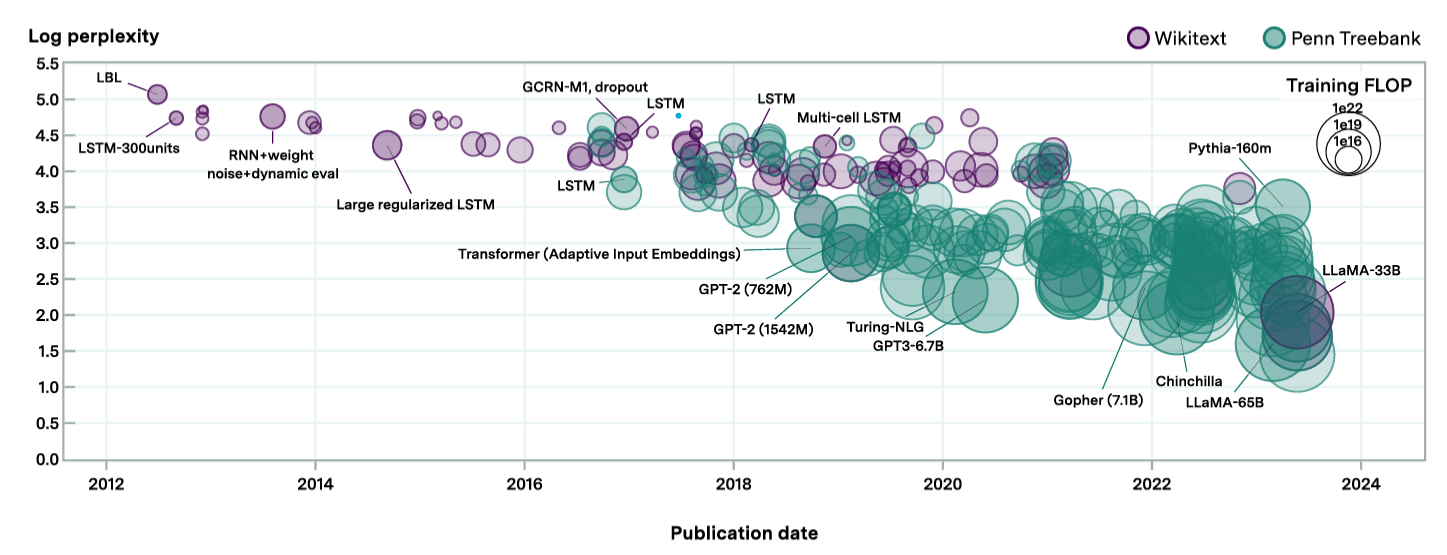
\includegraphics[width=0.9\textwidth]{images/compute_scaling.png}
    \caption{Performance in \textbf{language modeling} -- predicting the continuation of a sentence --, evaluated here in terms of \textbf{perplexity}, has steadily improved, while the size of the models has constantly increased. The increase in performance is also matched by equivalent data scaling, with variations in modelling becoming asymptotically less significant. Reproduced from \cite{ho2024algorithmic}.}
    \label{fig:compute_scaling}
\end{figure}

If we take scaling laws as given, we are left with an almost magical tool. In a nutshell, neural networks are optimized to approximate some probability distribution given data drawn from it. In principle, this approximation may fail: for example, modern neural networks are so large that they can easily memorize all the data they are shown \cite{zhang2021understanding} and transform into a trivial look-up table. Instead, trained models are shown to generalize well even to tasks that are not explicitly considered in the training data \cite{akyurek2022learning}. In fact, as the size of the datasets increases, the concept of what is \textit{in-distribution} and what is \textit{out-of-distribution} blurs, and large-scale models show hints of strong generalization capabilities and a fascinating low dependency on pure memorization, i.e., \textbf{overfitting} \cite{power2022grokking}. 

The emergence of extremely large models that can be leveraged for a variety of downstream tasks (sometimes called \textbf{foundation models}), coupled with a vibrant open-source community,\footnote{\url{https://huggingface.co/}} has also shifted how we interact with these models. Many tasks can now be solved by simply \textit{prompting} (i.e., interacting with text or visual instructions) a pre-trained model found on the web \cite{akyurek2022learning}, with the internals of the model remaining a complete black-box. From a high-level perspective, this is similar to a shift from having to programs your libraries in, e.g., C++, towards relying on open-source or commercial software whose source code is not accessible. The metaphor is not as far fetched as it may seems: nowadays, few teams worldwide have the compute and the technical expertise to design and release truly large-scale models such as the Llama LLMs \cite{touvron2023llama}, just like few companies have the resources to build enterprise CRM software.

And in the same way, just like open-source software provides endless possibilities for customizing or designing from scratch your programs, customer-grade hardware and a bit of ingenuity gives you a vast array of options to experiment with differentiable models, from \textbf{fine-tuning} them for your tasks \cite{liu2022few} to merging different models \cite{ainsworth2022git}, quantizing them for low-power hardware, testing their robustness, or even designing completely new variants and ideas. For all of this, you need to look `under the hood'  and understand how these models process and manipulate data internally, with all their tricks and idiosincrasies that are born from experience and debugging. This book is an entry point into this world: if, like Alice, you are naturally curious, I hope you will appreciate the journey.

\section*{About this book}

We assume our readers are familiar with the basics of \textbf{machine learning} (ML), and more specifically \textbf{supervised learning} (SL). SL can be used to solve complex tasks by gathering data on a desired behavior, and `training' (optimizing) systems to approximate that behavior. This deceptively simple idea is extremely powerful: for example, image generation can be turned into the problem of collecting a sufficiently large collection of images with their captions; simulating the English language becomes the task of gathering a large collection of text and learning to predict a sentence from the preceding ones; and diagnosing an X-ray becomes equivalent to having a large database of scans with the associated doctors’ decision (Figure \ref{fig:examples}).

\begin{figure}
    \centering
    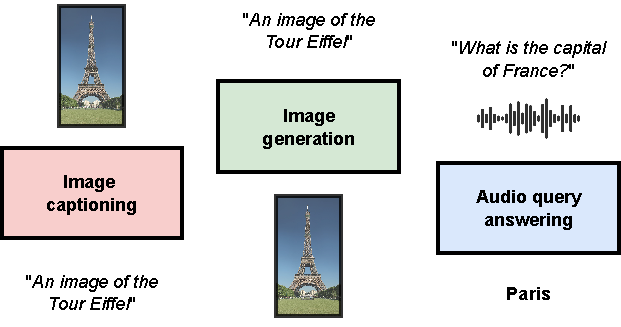
\includegraphics[width=0.6\textwidth]{images/examples.pdf}
    \caption{Most tasks can be categorized based on the desired input - output we need: {\color{drawgreen}image generation} wants an image (an \textit{ordered grid} of pixels) from a text (a \textit{sequence} of characters), while the inverse ({\color{drawred}image captioning}) is the problem of generating a caption from an image. As another example, {\color{drawblue}audio query answering} requires a text from an audio (another \textit{ordered} sequence, this time numerical). Fascinatingly, the design of the models follow similar specifications in all cases.}
    \label{fig:examples}
\end{figure}

In general, learning is a \textbf{search} problem. We start by defining a program with a large number of \textit{degree-of-freedoms} (that we call parameters), and we manipulate the parameters until the model performance is satisfying. To make this idea practical, we need efficient ways of searching for the optimal configuration even in the presence of millions (or billions, or trillions) of such parameters. As the name implies, \textbf{differentiable models} do this by restricting the selection of the model to differentiable components, i.e., mathematical functions that we can differentiate. Being able to compute a derivative of a high-dimensional function (a gradient) means knowing what happens if we slightly perturb their parameters, which in turn leads to automatic routines for their optimization (most notably, \textbf{automatic differentiation} and \textbf{gradient descent}). Describing this setup is the topic of the first part of the book (Part \ref{part:compass_and_needle}, \textbf{Compass and Needle}), going from Chapter \ref{chap:preliminaries} to Chapter \ref{chap:automatic_differentiation}.

By viewing neural networks as simply compositions of differentiable primitives we can ask two basic questions (Figure \ref{fig:differentiable_programming}): first, what \textbf{data types} can we handle as inputs or outputs? And second, what sort of primitives can we use? Differentiability is a strong requirement that does not allow us to work directly with many standard data types, such as characters or integers, which are fundamentally \textit{discrete} and hence discontinuous. By contrast, we will see that differentiable models can work easily with more complex data represented as large arrays (what we will call \textbf{tensors}) of numbers, such as images, which can be manipulated algebraically by basic compositions of linear and nonlinear transformations. 

In the second part of the book we focus on a prototypical example of differentiable component, the \textbf{convolutional} operator (Part \ref{part:a_strange_land}, from Chapter \ref{chap:cnns} until Chapter \ref{chap:deep_cnns}). Convolutions can be applied whenever our data can be represented by an ordered sequence of elements: these include, among others, audio, images, text, and video. Along the way we also introduce a number of useful techniques to design \textit{deep} (a.k.a., composed of many steps in sequence) models, as long as several important ideas such as \textbf{text tokenization}, \textbf{autoregressive} generation of sequences, and \textbf{causal} modeling, which form the basis for state-of-the-art LLMs. 

\begin{SCfigure}
    \centering
    \hspace{1em}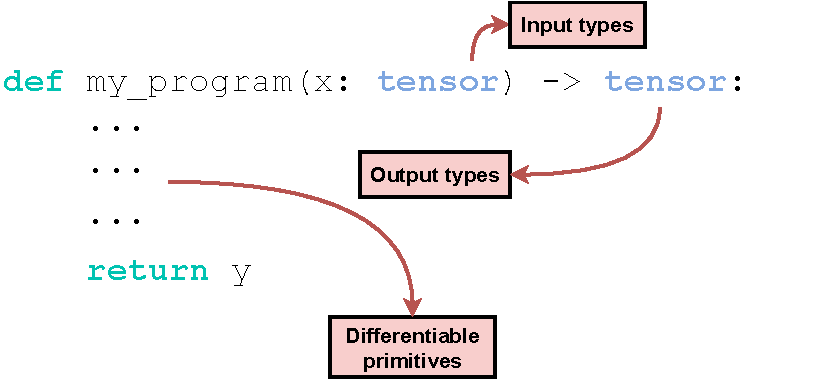
\includegraphics[width=0.6\textwidth]{images/differentiable_programming.pdf}
    \caption{Neural networks are sequences of differentiable \textbf{primitives} which operate on structured arrays (\textbf{tensors}): each primitive can be categorized based on its input/output signature, which in turn defines the rules for composing them.}
    \label{fig:differentiable_programming}
\end{SCfigure}

The third part of the book (Part \ref{part:down_the_rabbit_hole}, \textbf{Down the Rabbit Hole}) continues our exploration of differentiable models by considering alternative designs for sets (most importantly \textbf{attention} layers and \textbf{transformer} models in Chapter \ref{chap:transformers} and \ref{chap:transformers_in_practice}), graphs (Chapter \ref{chap:gnns}), and finally recurrent layers for temporal sequences (Chapter \ref{chap:rnns}). 

The book is complemented by a website\footnote{\url{https://sscardapane.it/alice-book}} where I collect additional chapters and material on topics of interest that do not focus on a specific type of data, including \textbf{generative modelling}, \textbf{conditional computation}, \textbf{transfer learning}, and \textbf{explainability}. These chapters are more research-oriented in nature and can be read in any order. Hopefully they will be part of a second volume if time allows.
%
\section*{What is ``differentiable programming''?}

Neural networks have a long and rich history. The name itself is a throwback to early attempts at modelling (biological) neurons in the 20th century, and similar terminology has remained pervasive: to be consistent with existing frameworks, in the upcoming chapters we may refer to \textit{neurons}, \textit{layers}, or, e.g., \textit{activations}. After multiple waves of interest, the period between 2012 and 2017 saw an unprecedented rise in complexity in the networks spurred by large-scale benchmarks and competitions, most notably the \textbf{ImageNet Large Scale Visual Recognition Challenge} (ILSVRC) that we cover in Chapter \ref{chap:deep_cnns}. A second major wave of interest came from the introduction of \textbf{transformers} (Chapter \ref{chap:transformers}) in 2017: just like computer vision was overtaken by convolutional models a few years before, natural language processing was overtaken by transformers in a very short period. Further improvements in these years were done for videos, graphs (Chapter \ref{chap:gnns}), and audio, culminating in the current excitement around LLMs, multimodal networks, and generative models.\footnote{This is not the place for a complete historical overview of modern neural networks; for the interested reader, I refer to \cite{metz2022genius} as a great starting point.}

This period paralleled a quick evolution in terminology, from the \textbf{connectionism} of the 80s \cite{rumelhart1986general} to the use of \textbf{deep learning} for referring to modern networks in opposition to the smaller, \textit{shallower} models of the past \cite{bengio2009learning,lecun2015deep}. Despite this, all these terms remain inexorably vague, because modern (artificial) networks retain almost no resemblance to biological neural networks and neurology \cite{zador2023catalyzing}. Looking at modern neural networks, their essential characteristic is being composed by differentiable blocks: for this reason, in this book I prefer the term \textbf{differentiable models} when feasible. Viewing neural networks as differentiable models leads directly to the wider topic of \textbf{differentiable programming}, an emerging discipline that blends computer science and optimization to study differentiable computer programs more broadly \cite{blondel2024elements}.\footnote{Like many, I was inspired by a `manifesto' published by Y. LeCun on Facebook in 2018: \url{https://www.facebook.com/yann.lecun/posts/10155003011462143}. For the connection between neural networks and open-source programming (and development) I am also thankful to a second manifesto, published by C. Raffel in 2021: {\url{https://colinraffel.com/blog/a-call-to-build-models-like-we-build-open-source-software.html}}.}

As we travel through this land of differentiable models, we are also traveling through history: the basic concepts of numerical optimization of linear models by gradient descent (covered in Chapter \ref{chap:linear_models}) were known since at least the XIX century \cite{stigler1981gauss}; so-called ``fully-connected networks'' in the form we use later on can be dated back to the 1980s \cite{rumelhart1986general}; convolutional models were known and used already at the end of the 90s \cite{lecun1998gradient}.\footnote{For a history of NNs up to this period through interviews to some of the main characters, see \cite{anderson2000talking}; for a large opinionated history there is also an \textit{annotated history of neural networks} by J. Schmidhuber: \url{https://people.idsia.ch/~juergen/deep-learning-history.html}.} However, it took many decades to have sufficient data and power to realize how well they can perform given enough data and enough parameters.

\begin{figure}
    \centering
    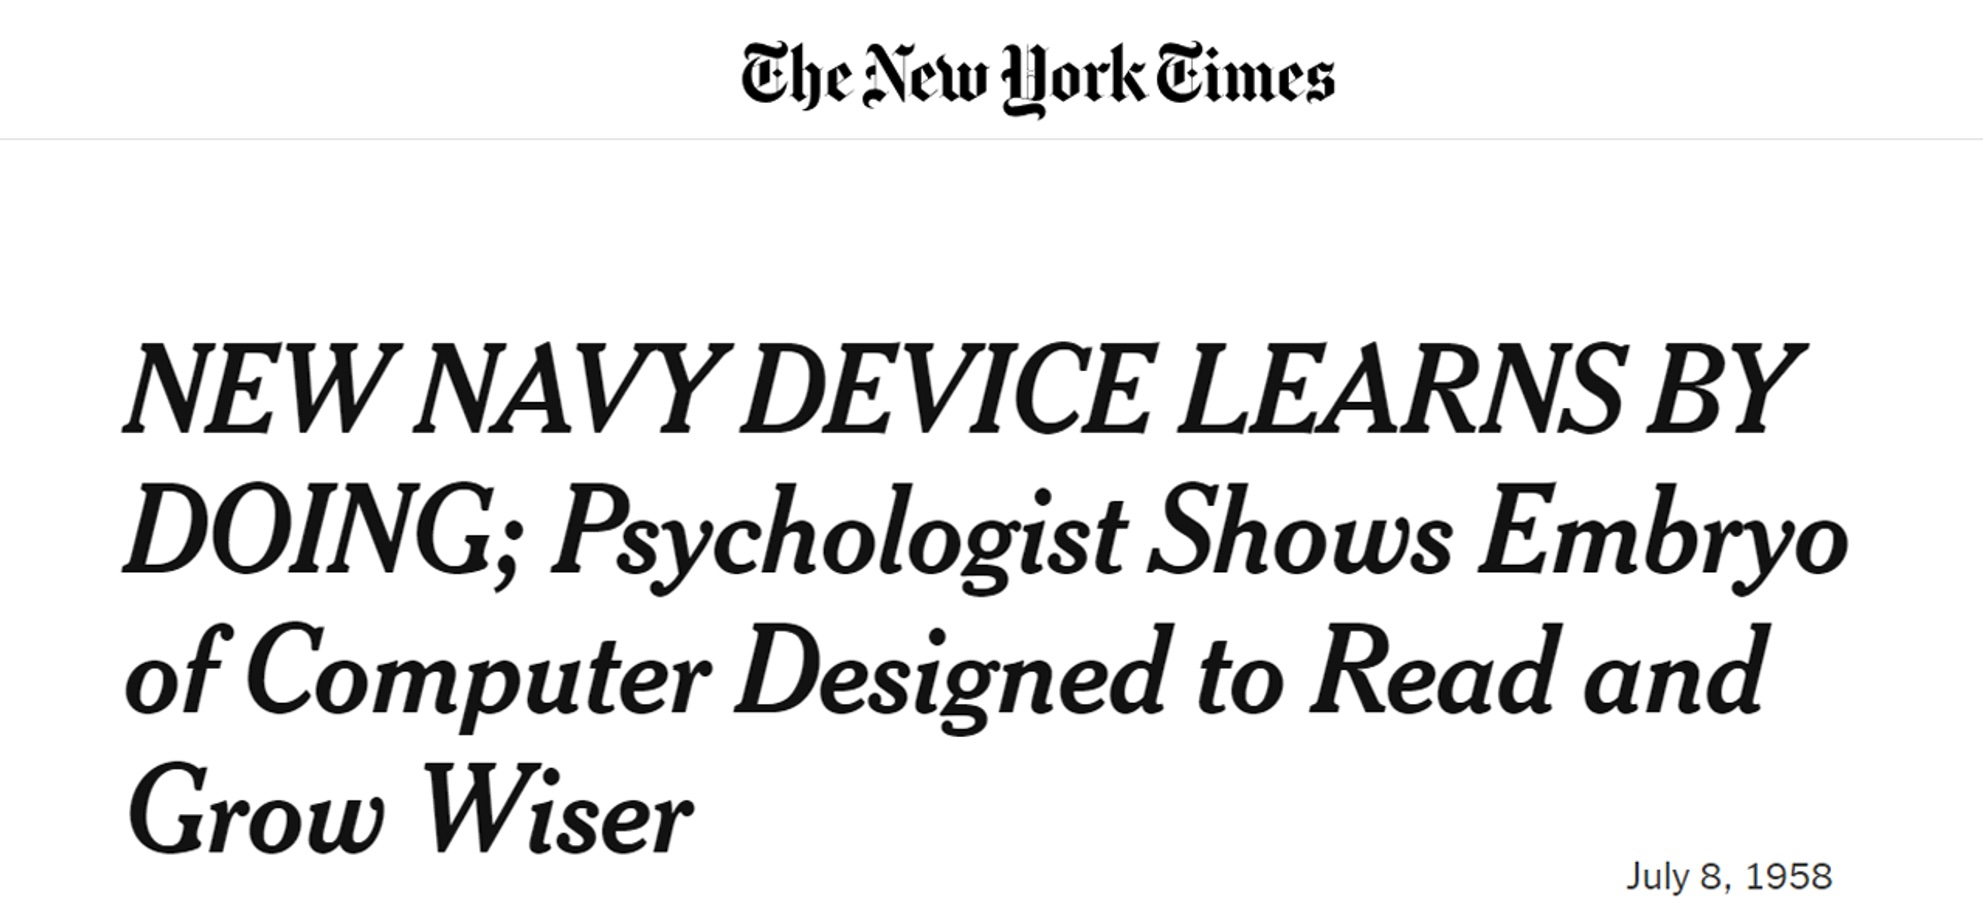
\includegraphics[width=0.7\textwidth]{images/Rosenblatt_cut.jpg}
    \caption*{AI hype - except it is 1958, and the US psychologist Frank Rosenblatt has gathered up significant media attention with his studies on ``perceptrons'', one of the first working prototypes of neural networks.}
\end{figure}

While we do not have space to go in-depth on all possible topics (also due to how quickly the research is progressing), I hope the book provides enough material to allow the reader to easily navigate the most recent literature.

\section*{Notation and symbols}
\label{sec:notation}

\begin{figure}
    \centering
    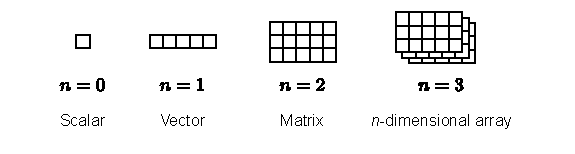
\includegraphics[width=0.9\textwidth]{images/Tensors.pdf}
    \caption*{Fundamental data types: scalars, vectors, matrices, and generic $n$-dimensional arrays. We use the name \textbf{tensors} to refer to them. $n$ is called the \textbf{rank} of the tensor. We show the vector as a row for readability, but in the text we assume all vectors are \textit{column} vectors.}
\end{figure}

The fundamental data type when dealing with differentiable models is a \textbf{tensor},\footnote{In the scientific literature, tensors have a more precise definition as multilinear operators \cite{lim2021tensors}, while the objects we use in the book are simpler multidimensional arrays. Although technically a misnomer, the use of \textit{tensor} is so widespread that we keep this convention here.} which we define as an $n$-dimensional array of objects, typically real-valued numbers. With the necessary apology to any mathematician reading us,\footnote{Assuming anyone is actually reading us.} we call $n$ the \textbf{rank} of the tensor. The notation in the book varies depending on $n$:
%
\begin{itemize}
    \item A single-item tensor ($n=0$) is just a single value (a \textbf{scalar}). For scalars, we use lowercase letters, such as $x$ or $y$.\footnote{If you are wondering, scalars are named like this because they can be written as scalar multiples of one. Also, I promise to reduce the number of footnotes from now on.}
    \item Columns of values ($n=1$) are called \textbf{vectors}. For vectors we use a lowercase bold font, such as $\mathbf{x}$. The corresponding row vector is denoted by $\mathbf{x}^\top$ when we need to distinguish them. We can also ignore the transpose for readability, if the shape is clear from context.
    \item Rectangular array of values ($n=2$) are called a \textbf{matrix}. We use an uppercase bold font, such as $\mathbf{X}$ or $\mathbf{Y}$.
    \item No specific notation is used for $n > 2$. We avoid calligraphic symbols such as $\mathcal{X}$, that we reserve for sets or probability distributions.
\end{itemize}
%
For working with tensors, we use a variety of indexing strategies described better in Section \ref{sec:linear_algebra}. In most cases, understanding an algorithm or an operation boils down to understanding the shape of each tensor involved. To denote the shape concisely, we use the following notation:
%
$$
X \sim(b,h,w,3)
$$
%
This is a rank-$4$ tensor with shape $(b,h,w,3)$. Some dimensions can be pre-specified (e.g., $3$), while other dimensions can be denoted by variables. We use the same symbol to denote drawing from a probability distribution, e.g., $\varepsilon \sim \mathcal{N}(0,1)$, but we do this rarely and the meaning of the symbol should always be clear from context. Hence, $\mathbf{x} \sim (d)$ will substitute the more common $\mathbf{x} \in \mathbb{R}^d$, and similarly for $\mathbf{X} \sim (n,d)$ instead of $\mathbf{X} \in \mathbb{R}^{n \times d}$.
%
Finally, we may want to constrain the elements of a tensor, for which we use a special notation:
%
\begin{enumerate}
    \item $\mathbf{x} \sim \text{Binary}(c)$ denotes a tensor with only binary values, i.e., elements from the set $\left\{0,1\right\}$.
    \item $\mathbf{x} \sim \Delta(a)$ denotes a vector belonging to the so-called \textbf{simplex}, i.e., $x_i \ge 0$ and $\sum_i x_i = 1$. For tensors with higher rank, e.g., $\mathbf{X} \sim \Delta(n,c)$, we assume the normalization is applied with respect to the last dimension (e.g., in this case each row of $\mathbf{X}_i$ belongs to the simplex).
\end{enumerate}
%
Additional notation is introduced along each chapter when necessary. We also have a few symbols on the side: 

\begin{itemize}
\item  \addbottle A \textbf{bottle} to emphasize some definitions. We have many definitions, especially in the early chapters, and we use this symbol to visually discriminate the most important ones.
\item \addclock A \textbf{clock} for sections we believe crucial to understand the rest of the book -- please do not skip these!
\item \addteacup On the contrary, a \textbf{teacup} for more relaxed sections -- these are generally discursive and mostly optional in relation to the rest of the book.
\end{itemize}

\section*{Final thoughts before departing}

The book stems from my desire to give a coherent form to the lectures I prepared for a course called \textbf{Neural Networks for Data Science Applications}, which I have been teaching in the Master Degree in Data Science at Sapienza University of Rome for a few years. The core chapters of the book constitute the main part of the course, while the remaining chapters are topics that I cover on and off depending on the year. Some parts have been supplemented by additional courses I have taught (or I intend to teach), including parts of \textbf{Neural Networks} for Computer Engineering, an introduction to machine learning for Telecommunication Engineering, plus a few tutorials, PhD courses, and summer schools over the years.

There are already a number of excellent (and recent) books on the topic of modern, deep neural networks, including \cite{prince2023understanding, zhang2023dive,bishop2024deep,fleuret2023little,hardt2022patterns}. This book covers a similar content to all of these in the beginning, while the exposition and some additional parts (or a few sections in the advanced chapters) intersect less, and they depend mostly on my research interests. I hope I can provide an additional (and complementary) viewpoint on existing material.

% As a rule, I believe it is important to understand why and how certain equations come to be, especially in a field such as neural networks, where untold questions must be answered with \textit{because it works best this way} or \textit{historically it has been like this}. Hence, I have tried to provide a simple formalism with enough rigor, while giving insights when possible into each and every concept that I introduce. In general, I have avoided theorems, proofs, or analyses of convergence or approximation. There are much better resources in this regard than I can provide.

As my choice of name suggests, understanding differentiable \textit{programs} comes from both theory and coding: there is a constant interplay between how we design models and how we implement them, with topics like automatic differentiation being the best example. The current resurgence of neural networks (roughly from 2012 onwards) can be traced in large part to the availability of powerful software libraries, going from Theano \cite{al2016theano} to Caffe, Chainer, and then directly to the modern iterations of TensorFlow, PyTorch, and JAX, among others. I try whenever possible to connect the discussion to concepts from existing programming frameworks, with a focus on PyTorch and JAX. The book is not a programming manual, however, and I refer to the documentation of the libraries for a complete introduction to each of them. 

Before moving on, I would like to list a few additional things this book \textit{is not}. First, I have tried to pick up a few concepts that are both (a) common today, and (b) general enough to be of use in the near future. However, I cannot foresee the future and I do not strive for completeness, and several parts of these chapters may be incomplete or outdated by the time you read them. Second, for each concept I try to provide a few examples of variations that exist in the literature (e.g., from batch normalization to layer normalization). However, keep in mind that hundreds more exist: I invite you for this to an exploration of the many pages of \href{http://paperswithcode.com}{Papers With Code}. Finally, this is a book on the fundamental components of differentiable models, but implementing them at scale (and making them work) requires both engineering sophistication and (a bit of) intuition. I cover little on the hardware side, and for the latter nothing beats experience and opinionated blog posts.\footnote{See for example this blog post by A. Karpathy: \url{http://karpathy.github.io/2019/04/25/recipe/}, or his recent \textbf{Zero to Hero} video series: \url{https://karpathy.ai/zero-to-hero.html}.}

\section*{Acknowledgments}
%
Equations' coloring is thanks to the beautiful {\footnotesize\verb+st--/annotate-equations+}
package.\footnote{\url{https://github.com/st--/annotate-equations/tree/main}} Color images of Alice in Wonderland and the black and white symbols in the margin are all licensed from Shutterstock.com. The images of Alice in Wonderland in the figures from the main text are reproductions from the original Arthur Rackham's 1907 illustrations, thanks to Wikimedia.\footnote{\url{ https://commons.wikimedia.org/wiki/Category:Alice\%27s\_adventures\_in\_Wonderland\_(Rackham,\_1907)}} I thank Roberto Alma for extensive feedback on a previous draft of the book and for encouraging me to publish the book. I also thank Corrado Zoccolo and Emanuele Rodolà for providing corrections and suggestions to the current version, and everyone who provided me feedback via email.